\section{701 --- Insert into a Binary Search Tree}
Given the root node of a binary search tree (BST) and a value to be inserted into the tree, insert the value into the BST. Return the root node of the BST after the insertion. It is guaranteed that the new value does not exist in the original BST.

Note that there may exist multiple valid ways for the insertion, as long as the tree remains a BST after insertion. You can return any of them.

For example, 

Given the tree:

\begin{figure}[H]
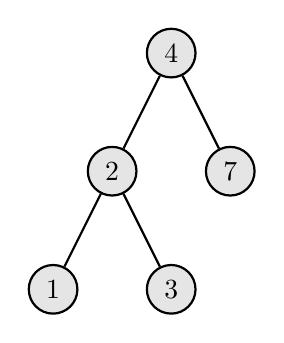
\begin{tikzpicture}
[every node/.style={draw, circle, fill=gray!20!, minimum size=5mm}, 
thick]
\node{4}
child{node{2} child{node{1}} child{node{3}}}
child{node{7}};
\end{tikzpicture}
\end{figure}

And the value to insert: 5

You can return this binary search tree:

\begin{figure}[H]
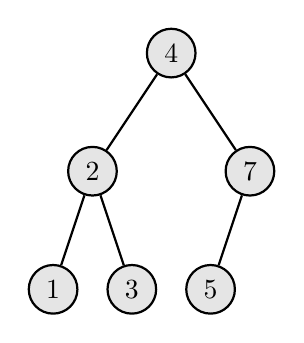
\begin{tikzpicture}
[every node/.style={draw, circle, fill=gray!20!, minimum size=5mm}, 
level 1/.style={sibling distance=20mm},
level 2/.style={sibling distance=10mm},
thick]
\node{4}
child{node{2} child{node{1}} child{node{3}}}
child{node{7} child{node{5}} child[missing]};
\end{tikzpicture}
\end{figure}

This tree is also valid:

\begin{figure}[H]
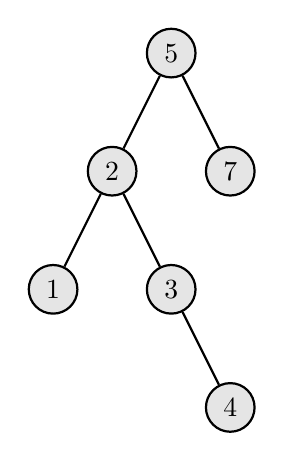
\begin{tikzpicture}
[every node/.style={draw, circle, fill=gray!20!, minimum size=5mm},
thick]
\node{5}
child{node{2} child{node{1}} child{node{3} child[missing] child{node{4}}}}
child{node{7}};
\end{tikzpicture}
\end{figure}

\subsection{Recursion}
Notice this is insertion not deletion. 

So, the approach is simple we can always insert new node as a child of the leaf. To define which leaf to use, we follow the standard BST logic :


\begin{itemize}
\item If \fcj{val > node.val}, go to insert into the right subtree.
\item If \fcj{val < node.val}, go to insert into the left subtree.
\end{itemize}

\setcounter{lstlisting}{0}
\begin{lstlisting}[style=customc, caption={Recursion}]
TreeNode* insertIntoBST( TreeNode* root, int val )
{
    if( !root )
    {
        return new TreeNode( val );
    }

    if( val < root->val )
    {
		//insert into left child
        root->left = insertIntoBST( root->left, val );
    }
    else
    {
		//insert into right child
        root->right = insertIntoBST( root->right, val );
    }

    return root;
}
\end{lstlisting}



